\section{Bewertung der Kraftwerksreserven zur Netzstabilisierung und Reserveleistungsvorhaltung}

Im vorherigen Kapitel wurden die verschiedene Reserven in Deutschland beleuchtet und definiert. Außerdem fand eine erste Bewertung der aktuellen Situation statt. Im folgenden sollen nun die technische und logistische Realisierbarkeit bzw. Nutzbarkeit der verschiedenen Reserven beleuchetet werden. Außerdem soll ein Ausblick auf zukünftige Entwicklungen, Möglichkeiten und Gefahren gegeben werden.

Dabei spielt auch der russische Überfall auf die Ukraine eine Rolle. Dieser wird in einer Aufnahme der momentanen deutschen Strategie zur Versorgungssicherheit im Winter berücksichtigt.

	\subsection{Bewertung der logistischen Situation der Reserven}
	Die Erhebung der Daten im Punkt Logistik gestaltet sich als herausfordernd. Hier gibt es das Problem, dass keine unabhängige Stelle die logistische Situation überwacht. Aussagen können nur von den Kraftwerksbetreibern selbst getätigt werden.
	
		\subsubsection{Logistischer Stand bei der Braunkohle (Arbeitstitel)} \label{sect: Braunkohle}
	Braunkohlekraftwerke befinden sich in Deutschland ausschließlich in der Sicherheitsbereitschaft. Die zwei Betreiber sind die RWE Power AG mit den zwei Blöcken Niederaußem E und F in Bergheim und dem Block Neurath C in Grevenbroich im Rheinischen Braunkohlerevier und die Lausitzer Energie und Kraftwerke AG, im folgenden LEAG, mit den zwei Blöcken Jänschwalde E und F in Teichland im Lausitzitzer Braunkohlerevier. \cite{Excel_Kraftwerksliste} \\
	
	Die Blöcke des Kraftwerks Jänschwalde werden durch Tagebaue der LEAG in Jänschwalde, Welzow-Süd, Nochten und Reichwalde versorgt. Der Transport wird auf der Schiene durch einen firmeneigenen Eisenbahnbetrieb realisiert. Der Abbau des Tagebaus Jänschwalde stoppt voraussichtlich im Jahr 2023. Dann ist der Tagebau erschöpft. Die Versorgung wird dann von den übrigen drei Abbaustandorten übernommen.
	Da es sich beim Kraftwerk Jänschwalde um ein Großkraftwerk mit 6 Blöcken handelt, welches inzwischen wieder aktiv am Strommarkt agiert, gibt es kein Personalproblem.\cite{LEAG_Braunkohleversorgung} \\
	
	Die in Sicherheitsbereitschaft befindlichen Blöcke Niederaußem E und F sowie Neurath C werden ebenfalls durch RWE-eigene Tagebaue versorgt. Hierbei handelt es sich um die Förderstätten Garzweiler, Hambach und Inden. Der Transport erfolgt über eine Eisenbahngesellschaft der RWE. Auch bei diesen drei Blöcken handelt es sich um Teile von größeren Kraftwerkskomplexen. Auch die Kraftwerksblöcke der RWE Power AG nehmen wieder aktiv am Strommarkt teil.  Daher stellt die Personalsituation kein Problem dar. \cite{Mail_RWE}
	
	\subsubsection{Logistischer Stand bei der Steinkohle} \label{sect: Steinkohle}
	Die deutschen Steinkohlekraftwerke, welche nicht mehr aktiv am Markt teilnehmen und noch nicht endgültig stillgelegt sind, befinden sich in Deutschland in der Netzreserve. Diese ist durch das KVGB und Paragraph 13b des EnWG rechtlich verankert. Bei den Betreibern handelt es sich um die EnBW Energie Baden-Würtemberg AG, die STEAG, Uniper Kraftwerke GmbH, Kraftwerk Mehrum GmbH und das Großkraftwerk Mannheim.\cite{Excel_Kraftwerksliste} \\
	
	Die logistische Situation war und ist angespannt. Niedrige Pegelstände von Rhein und Neckar, sowie der fehlende Gleisausbau in Deutschland erschwerten den Steinkohletransport deutlich. Die RAG Deutsche Steinkohle AG war der alleinige Betreiber deutscher Steinkohlebergwerke. Diese stellte den Abbau 2018 komplett ein, da dieser nicht mehr wirtschaftlich war. Damit sind die Betreiber zu \SI{100}{\percent} auf Importe angewiesen.\cite{Ende_Steinkohle}\\
	
	Die EnBW mit den Standorten Heizkraftwerk Altbach/Deizisau HKW 1, Heizkraftwerk Heilbronn HLB 5 und 6 sowie dem Kraftwerk Walheim mit den Blöcken 1 und 2 verstärkt seit Juli 2022 ihre Bemühungen zur Beschaffung, sowie der Erschließung von Flächen zur zusätzlichen Lagerung von Steinkohle. Auch die Personalsituation ist angespannt, da diese langfristig mit der Premisse der Stillegung geplant war. Die fünf Blöcke, welche sich in Netzreserve befinden, werden jedoch aller Voraussicht nach nicht wieder am Markt teilnehmen. Diese können nach eigener Aussage der EnBW aus technischen Gründen nicht ununterbrochen zur Stromerzeugung eingesetzt werden. Grund hierfür ist das fortgeschrittene Alter der Anlagen.\cite{EnBW_Steinkohle} \\
	
	Der Stromerzeuger STEAG betreibt zwei Kraftwerke in Netzreserve, die Standorte Boxberg und Weiher 3 im Saarland. Die herausfordernde Lage der Kohleversorgung, auch mit hinblick auf den kommenden Winter, veranlasste das Wirtschaftsministerium des Saarlandes zu einem Logistik-Gipfel. Zu den Teilnehmenden gehörten unter Anderen der Staatssektretär des Bundesministeriums für Digitales und Verkehr, die STEAG selbst und die DB Cargo. Die Gespräche ergaben eine vorrangige Behandlung von Kohletransporten auf der Schiene gegenüber dem öffentlichen Personennahverkehr, im Falle von Versorgungsengpässen.\cite{Logistikgipfel_Saarland} Dies sichert die Belieferung der Kraftwerke mit Brennstoff. Zusätzlich tritt das Kraftwerk Boxberg zum 28.10.2022 wieder in den Markt ein. Das Schwesterkraftwerk Weiher 3 folgt am 31.10.2022. Ermöglicht wird dies durch das EKBG welches eine Rückkehr in den Strommarkt bis Frühjahr 2024 gestattet.\cite{STEAG_Steinkohle} \\
	
	
	\subsubsection{Logistischer Stand beim Gas}
	In Folge des russischen Überfalls auf die Ukraine sanken die deutschen Erdgasimporte aus Russland im September nach Stand 03.11.2022 auf null. Zum 03.05.2022 startete die Bundesnetzagentur eine Datenerhebung um den deutschen Gasverbrauch zu ermitteln.\cite{Datenerhebung_Gas} In einer Pressemitteilung vom 29.09.2022 wurde von einer notwendigen Einsparung in Höhe von \SI{20}{\percent} gesprochen um die Versorgungssicherheit auch von Erdgaskraftwerken im Winter zu gewährleisten, das Impulspapier von Acatech spricht sogar von 20 bis \SI{30}{\percent}.\cite{Impuls_Acatech_Einsparung}\\
	
	Deutsche Erdgaskraftwerke, welche nicht mehr im Betrieb sind, befinden sich sowohl in der Netz- als auch in der Kapazitätsreserve. Die Versorgung ist sehr stark von den Netzbetreibern abhängig und die Situation sehr schwer vorhersehbar. Deutschlands Gasspeicher sind Stand 13.12.2022 zu \SI{100}{\percent} gefüllt. Des weiteren sollen zum Jahreswechsel 22/23 zwei FSRU in Betrieb genommen werden.\cite{LNG_FSRU}
	Ein zusätzliches Problem bei der Versorgung besteht in der Ausrichtung der in Europa vorhandenen Gas-Infrastruktur. Diese ist durch den Aufbau auf einen Gastransport von Ost nach West ausgerichtet. Der Großteil der europäischen LNG-Terminals befindet sich in Westeuropa. Damit ist eine Umkehrung des Gasflusses notwendig. Dieser sogenannte Reverse-Flow wird ermöglicht, indem die Verdichterstationen umgebaut werden. Danach ist ein Gastransport in beide Richtungen bei voller Kapazität möglich.\cite{Impuls_Acatech_Reverse_Flow} \\
	
	Ein eventuelles Verbot der Verstromung von Gas ist im Notfallplan Gas beschrieben. Dieser ist in drei Teile aufgeteilt. Die Frühwarnstufe und die Alarmstufe lassen einen Eingriff des Gesetzgebers vorerst nicht zu. Er setzt auf marktbasierte Maßnahmen zur Regulierung der verbrauchten Gasmengen. \\
	
	Sollte die Notfallstufe verkündet werden, so behält sich der Staat, in Form von Bundesministerium für Wirtschaft und Klima und Bundesnetzagentur als Lastverteiler, vor, die Substitution von Erdgas durch andere Brennstoffe anzuordnen. Diese ist jedoch nur eine von verschiedenen möglichen Maßnahmen, die getroffen werden könnten. Es steht nicht fest, von welchen Steuermechanismen gebrauch gemacht wird, da die Situation, in der sich Deutschland befindet, eine bisher nie dagewesene ist. \cite{Notfallplan_Gas}
	
	\subsubsection{Logistischer Stand beim Öl}
	Im Rahmen der Ölkrise von 1973, bei der durch politisch motivierte Verknappung der Öllieferungen der Preis künstlich angehoben wurde, kam es zur ersten Ölknappheit der Geschichte der Bundesrepublik Deutschland. Daraufhin wurde 1974 die Internationale Energieagentur gegründet, welche eine zuverlässige Energieversorgung koordienieren sollte. Diese Empfahl die Einrichtung einer strategischen Ölreserve, zur Absicherung von eventuellen Lieferausfällen. Seit dem beherbergt Deutschland genug Öl, um den Gebäude-, Industrie-, Verkehrs- und Energiesektor für 90 Tage mit Öl zu versorgen.\cite{strat_Ölreserve_Geschichte}\\
	
	In Deutschland gibt es 6 Blöcke in 3 Kraftwerken, die sich in der Netzreserve befinden und mit Öl befeuert werden.\cite{Excel_Kraftwerksliste} Die Versorgung dieser ist über Pipelines und Öltanker gesichert.\\
	Die Kraftwerke Ingolstadt in Großmehring und Irsching werden durch die TAL-Pipeline, welche von Triest kommend den großteil des Südens Deutschlands versorgt, mit Mineralöl beliefert.\\
	Das Kraftwerk Marbach, Betrieben durch die EnBW, liegt ebenfalls im Süden Deutschlands und wird durch die Pipeline TAL versorgt. Bei Lieferausfällen besteht auch in beiden Fällen die Möglichkeit über die nahe gelegene Donau bzw Neckar versorgt zu werden, sofern diese genug Wasser führen und Schiffsverkehr zulassen. Sollte auch dieser Versorgungsweg ausfallen, so steht noch die strategische Ölreserve zur Verfügung. Diese garantiert eine Versorgung mit Ölprodukten über mindestens 90 Tage. Die tatsächliche Reserve in Deutschland ist jedoch größer.\\
	
	\begin{figure}[H]
		\centering
		\includegraphics[page=1, width=0.6\textwidth]{./anhang/Ölreserve.png}
		\caption{Vergleich von Ölreserven verschiedener europäischer Länder}
		\label{Abb. Strategische Ölreserve} \cite{IEA_Ölreserven}
	\end{figure}
		
		
	\subsection{Kapazitätssituation für den Winter 2022/23}
	Im ersten Halbjahr 2022 erzeugte Erdgas \SI{30,7} Mrd. {kWh} elektrischen Strom in Deutschland. Dies entspricht einem Anteil von \SI{11,7}{\percent} der Gesamterzeugung.\cite{Stromproduktion_Erdgas} Im Hinblick auf drohende Versorgungsengpässe lohnt sich hier die Betrachtung der Gegenmaßnahmen, die bis hier hin getroffen wurden. \\
	
		\subsubsection{Der zweite Stresstest zum Stromsystem}
		Im Rahmen des vom BMWK in Auftrag gegebenen Stresstests, sollten die Übertragungsnetzbetreiber verschiedene Szenarien für die Versorgungssicherheit im Winter 2022/23 analysieren. Dabei wurden die Gasversorgung, die Steinkohleversorgung und eventuell ausfallende Kapazitäten im Ausland in augenschein genommen.\\
		
		Ein zentraler Punkt der Analyse war die Annahme, dass Polen keinen Strom exportieren kann, da die Versorgung mit Steinkohle durch Lieferengpässe nicht möglich ist. Desweiteren wurde davon ausgegangen, dass Frankreich bis zum Winter nicht alle Kernkraftwerke an den Markt bringen kann. Diese waren auf Grund von zu hohen Temperaturen, Niedrigwasser, Wartungsarbeiten und Defekten im Sommer teilweise abgeschaltet worden.\cite{AKW_Frankreich} Außerdem geht die Studie im kritischsten der drei Szenarien davon aus, dass Süddeutschland und Österreich die vertraglich geregelte Redispatchleistung aus Gaskraftwerken nicht liefern können. \\
		
		Das Fazit zeigt, dass in den beiden kritischsten Situationen auch in Deutschland einige Stunden der Lastunterdeckung auftreten. Desweiteren wird gezeigt, dass die deutsche Redispatchleistung in keinem der drei Szenarien ausreicht. Ausländische Leistungen müssen heran gezogen werden. Der Streckbetrieb der deutschen Kernkraftwerke entspannt die Situation. Lastunterdeckungen können weitestgehend vermieden werden, der Bedarf an Redispatch sinkt ebenfalls.\cite{Stresstest} \\
		
		Die Empfehlungen der Übertragungsnetzbetreiber stehen auf fünf Säulen. Diese sollen die angespannte Versorgungssituation enspannen:
			\begin{itemize}
				\item Transportkapazitäten erhöhen
				\item Redispatch-Potential im Ausland fokusieren
				\item vertragliches Lastmanagement
				\item Reserven nutzbar machen
				\item Nutzung weiterer Kraftwerkskapazitäten absichern
			\end{itemize}
		
		\subsubsection{Umsetzung der Empfehlungen} \label{sect: Atomausstieg}
		Am 07.10.2022 wurde vom Bundesrat die Novelle zum Energiesicherheitsgesetzt 3.0 verabschiedet. Dieses baut auf verschiedene Säulen zur Anhebung der Kapazitäten der Stromerzeugung. \cite{EnSiG}
			\begin{itemize}
				\item Erhöhung der Stromproduktion aus Photovoltaikanlagen
				\item Anreize für die Verstromung von Biogas
				\item Erhöhung der Produktion von Windstrom
				\item Maßnahmen zur Beschleunigung des Netzausbaus
				\item Maßnahmen im LNG-Beschleunigungsgesetz
				\item Erleichterung für den Brennstoffwechsel
				\item Änderungen im Baugesetztbuch
			\end{itemize}
		
		Zur Erhöhung der Produktionskapazitäten wurde außerdem ein Streckbetrieb für 3 verbeibende deutsche Atomkraftwerke beschlossen. Die Meiler Isar 2, Neckar-Westheim 2 und Emsland werden bis maximal Mitte April am Netz behalten. Diese sollen zusätzlich die Gaskraftwerke entlasten und Netzengpässe abfedern.\cite{Laufzeitverlängerung}\\
		Wie in Abschnitt \ref{sect: Steinkohle} beschrieben, konnten Versorgungsengpässe bei der Steinkohle überwunden werden. Außerdem traten einzelne Reservekraftwerke zum Oktober wieder in den Markt ein. Insgesamt nehmen Kraftwerke mit einer Gesamtnettokapazität von \SI{2,25}{\giga \watt} wieder am Strommarkt teil.\\
		Auch die Braunkohlekraftwerke aus der Sicherheitsbereitschaft (siehe \ref{sect: Braunkohle}) nehmen inzwischen wieder aktiv am Markt teil, die Blöcke Niederaußem E, F und Neurath C zum 01.10.2022, Jänschwalde E zum 06.10.2022 und Jänschwalde F zum 15.10.2022. Diese summieren sich zu einer elektrischen Nettoleistung von \SI{1,886}{\giga \watt}.\cite{Wiedereintritt_Kraftwerke} \\
		
		
	\subsection{Wie entwickeln sich Kraftwerksreserven zukünftig}	
	Der menschgemachte Klimawandel stellt eine gigantische Bedrohung für das Leben auf der Erde dar. Die Energiewende und mit ihr die essentielle Veränderung des Strom-, Wärme und Verkehrssektors stellen Deutschland vor drastische Herausforderungen. Zur Erreichung des 1,5 Grad Ziels müssen alle Nationen weltweit ihre Emissionen bilanziell auf null reduzieren, also klimaneutral werden. Sollten in Deutschland keine Änderungen in Kraft treten, wäre das \SI{}{\COtwo}-Budget zur Einhaltung des 1,5 Grad Ziels Stand November 2022 in 6 Jahren und 8 Monaten erschöpft, das Budget für die Erreichung des 2 Grad Ziels in 24 Jahren und 5 Monaten. Diese Zeiträume zeigen, die Notwendigkeit des Handelns.\cite{CO2_Uhr} \\
	
	Dem Stromsektor kommt bei der Erreichung der Klimaziele eine gesonderte Bedeutung zu. Nicht nur bietet er den Grundstein für die Dekarbonisierung der übrigen Sektoren, sondern stellt auch heute den größten \SI{}{\COtwo}-Emittenten dar.\cite{Umweltbundesamt_Emissionen} Deshalb ist es wichtig fossile Energieträger sukzessive zu substituieren. Mit der Verankerung des Klimaschutzes zur Generationen- und Freiheitssicherung im Grundgesetz sind die jetzige aber auch künftige Regierungen verpflichtet die \SI{}{\COtwo}-Emissionen zu senken und schlussendlich klimaneutral zu werden. Dafür stellte die Ampel-Koalition im November 2021 ihren Koalitionsvertrag vor, der folgende Maßnahmen enthält\cite{Koalitionsvertrag}:
		\begin{itemize}
			\item Atomausstieg bis Ende 2022
			\item Kohleausstieg im Optimalfall bis 2030
			\item Errichtung moderner \SI{}{\H{_2}}-ready Gaskraftwerke
			\item Zulassung von 15 Millionen vollelektrischen PKW bis 2030
			\item Deckung von \SI{80}{\percent} des Bruttostrobedarfs aus erneuerbaren Energien bis 2030
			\item PV-Ausbau verpflichtend bei gewerblichen Neubauten
			\item PV-Ausbau auf \SI{200}{\giga \watt}
			\item Ausweisung von \SI{2}{\percent} der Landfläche für Windkraft
			\item Kapazitätserhöhung von Off-Shore Winkraft auf mindestens \SI{30}{\giga \watt} bis 2030, \SI{40}{\giga \watt} bis 2035 und \SI{70}{\giga \watt} bis 2045
			\item Elektrolysekapazität von \SI{10}{\giga \watt} bis 2030
		\end{itemize}
		Im Oktober 2022 verständigte sich die Regierung mit der RWE Generation SE und dem Wirtschaftsministerium Nordrhein-Westfalen auf einen vorzeitigen Braunkohleausstieg im Rheinischen Revier für 2030.\cite{Kohleausstieg_RWE} \\
		
		Um jetztige Zustände und künftige Entwicklungen bewerten zu können bieten Studien und Modelle die Möglichkeit die Energieversorgung der nächsten Generation zu skizzieren. In dieser Ausarbeitung werden im besonderen Maße die Studien "`Klimaneutrales Stromsystem 2035"' von Agora Energiewende, sowie die Studie "`Energiewende im Sozialen Raum"', einer Zusammenarbeit von Germanwatch, Global Climate Forum und dem Frauenhofer Institut für Energirwirtschaft und Energiesystemtechnik, welche auf Annahmen des "`Ariadne Report"' des Potsdam-Insitut für Klimafolgenforschung (PIK) fußt, in Augenschein genommen.\\

		\subsubsection{Wo befinden wir uns?}
		Im Rahmen der wirtschaftlichen Teilerholung im Jahr 2021 stiegen die \SI{}{\COtwo}-Emissionen um 33 Millionen Tonnen, davon 26 Millionen Tonnen verursacht durch die Energiewirtschaft, im vergleich zum Vorjahr an. Dies entspricht einem Anstieg von \SI{4,5}{\percent}.\cite[S.5]{Stand_der_Dinge} Grund dafür waren die erhöhten Primärenergieverbräuche der Industrie und Haushalte, sowie eine stärkere Kohleverstromung infolge der steigenden Gaspreise, welcher die Erzeugung von Strom aus Kohle wirtschaftlicher gestaltete. \ref{sect: Wie funktioniert der deutsche Strommarkt?} Auch der Anteil erneuerbarer Energien an der Stromproduktion sank um \SI{3}{\percent}, der größte Einbruch den Deutschland je zu verzeichnen hatte, auf \SI{42,3}{\percent}.\cite[S.5]{Stand_der_Dinge}\\
		
		Der Ausbau erneuerbarer Energien ging in diesem Zeitraum sehr langsam voran. So lag der Zubau bei lediglich \SI{6,7}{\giga \watt p}. Hiervon waren \SI{75}{\percent} Photovoltaik und \SI{25}{\percent} On-Shore Windkraft und Biomasseanlagen. Es wurde keine einzige Off-Shore Winkraftanlage in Betrieb genommen. \cite[S.47 ff.]{Stand_der_Dinge}
		
		
		\subsubsection{Entwicklung der Reserven bis 2030} \label{sect: 2030}
		Blickt man auf die bevorstehenden Veränderungen, lohnt sich die Frage, wie sich die Energieversorgung zukünftig entwickeln wird. Dieses Thema ist auch Gegenstand zahlreicher Studien. Zur möglichst qualifizierten Veraussage eines zukünftigen Versorgungssystems werden Szenarien und Modelle erstellt.\\
		
		Mit Hilfe des Szenarios "`Klimaneutrales Stromsystem 2035"' wird beschrieben, wie die ambitionierten Klimaziele der derzeitigen Bundesregierung möglichst Effizient umgesetzt werden können. Besagter Rahmen baut auf dem früher erschienenen Szenario "`Klimaneutrales Deutschland 2045"' auf, welches die Grundlage für die Berechnungen liefert.\\
		Die Annahmen der Studie liefert die Novellierung des EEG. Angenommen werden für das Jahr 2030 \SI{115}{\giga \watt} Onshore-Windkraft, \SI{30}{\giga \watt} Offshore-Windkraft und \SI{215}{\giga \watt} Photovoltaik.\cite[S.22]{Agora_KlimaneutralesStromsystem} Die restlichen Annahmen sind der Tabelle \ref{Abb. Annahmen Agora2035} zu entnehmen.	Es wird ein Bruttostromverbrauch von \SI{726}{\tera \watt \hour} angenommen.\cite[S.33]{Agora_KlimaneutralesStromsystem} Desweiteren wird 2030 der Kohleausstieg vollzogen, sodass ab dann nur noch Gaskraftwerke und Pumpspeicherkraftwerke als gesicherte Leistung zur Verfügung stehen.\cite[S.31]{Agora_KlimaneutralesStromsystem} \\
		
		\begin{figure}[H]
			\centering
			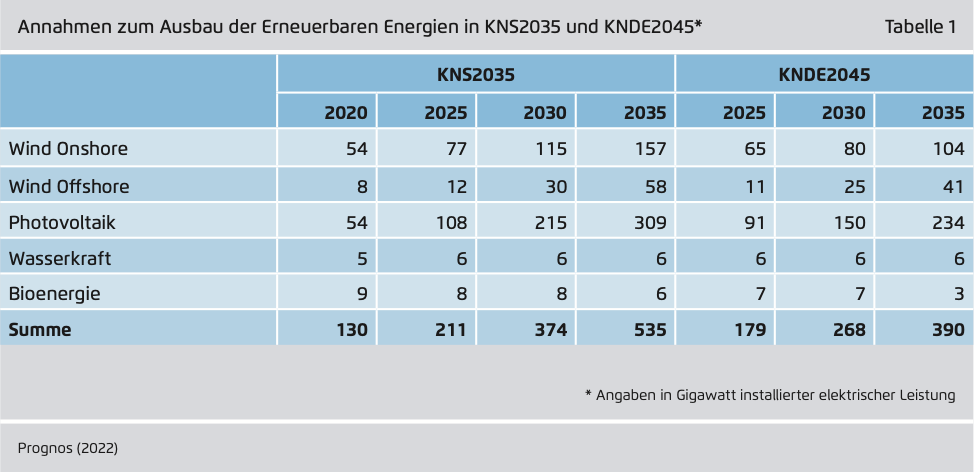
\includegraphics[page=1, width=0.6\textwidth]{./anhang/Annahmen Agora2035.png}
			\caption{Annahmen im Szenario}
			\label{Abb. Annahmen Agora2035} \cite[S.22]{Agora_KlimaneutralesStromsystem}
		\end{figure}
	
		Mit Erreichung der Ausbauziele läge in diesem Szenario der Anteil Erneuerbarer Energien an der Nettostromerzeugung, inklusive von Speichern und wasserstoffbasierter Energieerzeugung bei \SI{81,5}{\percent} und würde bis 2035 auf \SI{87}{\percent} ansteigen. \cite[S.23]{Agora_KlimaneutralesStromsystem} Zur Erreichung dieser Ziele muss der Ausbau erneuerbarer Energien an Geschwindigkeit gewinnen. Der notwendige jährliche Bruttozubau kann in den anschließenden Grafiken gefunden werden. \\
			
			\begin{figure}[H]
				\centering
				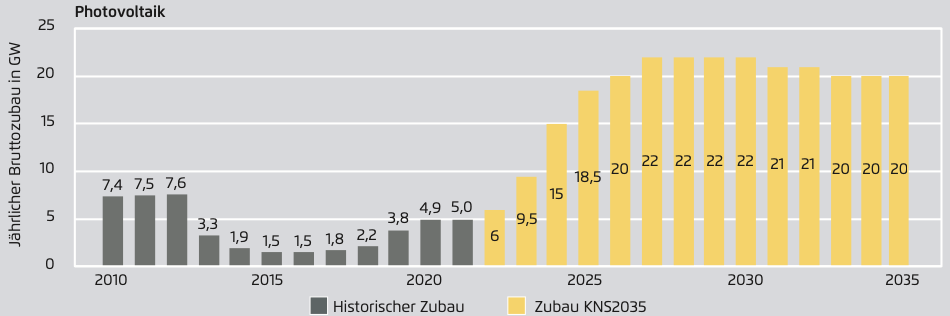
\includegraphics[page=1, clip, width=0.6\textwidth]{./anhang/Zubau PV Agora2035.png}
				\caption{Benötigter jährlicher Zubau PV}
				\label{Abb.Zubau PV Agora2035} \cite[S.24]{Agora_KlimaneutralesStromsystem}
			\end{figure}
			
				\begin{figure}[H]
				\centering
				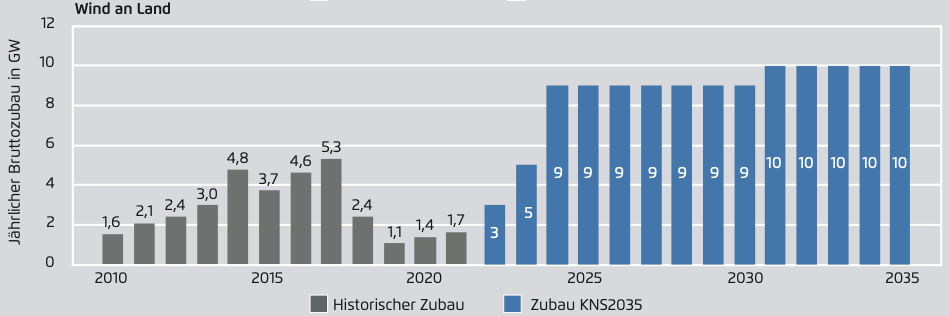
\includegraphics[page=1, clip, width=0.6\textwidth]{./anhang/Zubau Onshore Agora2035.png}
				\caption{Benötigter jährlicher Zubau Onshore Winkraft}
				\label{Abb.Zubau Onshore Agora2035} \cite[S.24]{Agora_KlimaneutralesStromsystem}
			\end{figure}
		
				\begin{figure}[H]
				\centering
				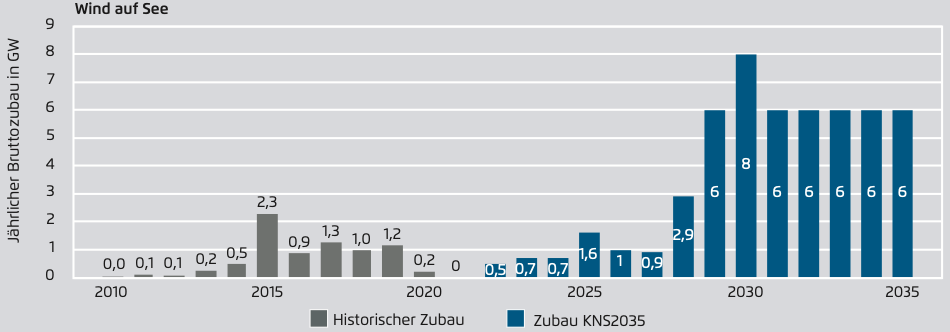
\includegraphics[page=1, clip, width=0.6\textwidth]{./anhang/Zubau Offshore Agora2035.png}
				\caption{Benötigter jährlicher Zubau Offshore Winkraft}
				\label{Abb.Zubau Offshore Agora2035} \cite[S.24]{Agora_KlimaneutralesStromsystem}
			\end{figure}
		Die volatilen erneuerbaren Energien können jedoch nicht allein für eine Versorgungssicherheit garantieren. Der Kraftwerksreserve wird in den kommenden Jahren eine zentrale Rolle zur Sicherung der Stromversorgung unabhängig von meteorologischen Bedingungen zukommen. Zur Abdeckung der Residuallast werden in den 2030er Jahren regelbare \SI{}{\H{_2}}-Ready Gaskraftwerke zum Einsatz kommen. Diese Kraftwerke müssen heute schon gebaut werden. Der Bauprozess benötigt von der Planung bis zur Inbetriebnahme 5 Jahre und die Anzahl der gleichzeitig baubaren Kraftwerke ist beschränkt.\\
		Die Gaskraftwerke werden zu Beginn noch mit Erdgas versorgt. Dieses wird jedoch in den folgenden Jahren durch Wasserstoff ersetzt. Bei benötigten \SI{61}{\giga \watt} installierter Leistung, von denen \SI{20}{\giga \watt} auf etwa 3300 Vollbelastungsstunden kommen und ein dreiviertel des produzierten Stroms erzeugen, wird ein Zubau von \SI{30}{\giga \watt} notwendig. \cite[S.9]{Agora_KlimaneutralesStromsystem} Dies entspricht in etwa 40 modernen Gaskraftwerken. Dabei ist die benötigte Infrastruktur zentral. Es wäre zu Überlegen, ob bei Spitzenlastkraftwerken mit nur wenigen Vollbelastungsstunden im Jahr und geringeren Wirkungsgraden ein Anschluss an das Wasserstoffnetz sinnvoll ist. Hier könnte auch auf besser Lager- und Transportierbare Derivate wie Ammoniak zurück gegriffen werden.\\
		
		Auch die Resourcen zur Frequenz- und Spannungshaltung werden sich künftig verändern. Die Atom-, Kohle und Ölkapazitäten müssen durch neue und vorhandene Gaskraftwerke ersetzt werden. Die heute schon viel verwendete Wasserkraft wird auch zukünftig zur Verfügung stehen.\\
		Im Falle einer Überproduktion von erneuerbarem Strom soll es künftig nur noch selten zu Abschaltung kommen. Vielmehr soll hier auf eine Flexibilisierung des Stromnetzes gesetzt werden. So kann nicht genutzter Strom über Elektrolyseure in grünen Wasserstoff umgewandelt und gespeichert werden. Hier soll die installierte elektrische Leistung 2030 \SI{12}{\giga \watt } betragen. \cite[S.11]{Agora_KlimaneutralesStromsystem} Die Platzierung der Elektrolysestationen an Netzengstellen verringert zudem die Menge an Redispatch-Leistung. Außerdem eröffnet die Elektrifizierung des Gebäude-, Industrie- und Verkehrssektors neue Möglichkeiten. So können Wärmepumpen in Zeiten hoher Erzeugung zugeschalten werden um nicht genutzten Strom in Wärme umzuwandeln und zu speichern. Ähnlich sollen elektrifizierte Industrieprozesse genutzt werden um Überschussstrom zu zwischenzuspeichern.\\
		Auch der Elektromobilität kommt eine neue Rolle zu. Die in batteriebetriebenen Elektroautos enthaltenen Speicher sollen den Strom sowohl elektrisch zwischenspeichern, als auch ins Netz abgeben können. Diesen Prozess nennt man Vehicle-to-Grid.\\
			
			\begin{figure}[H]
				\centering
				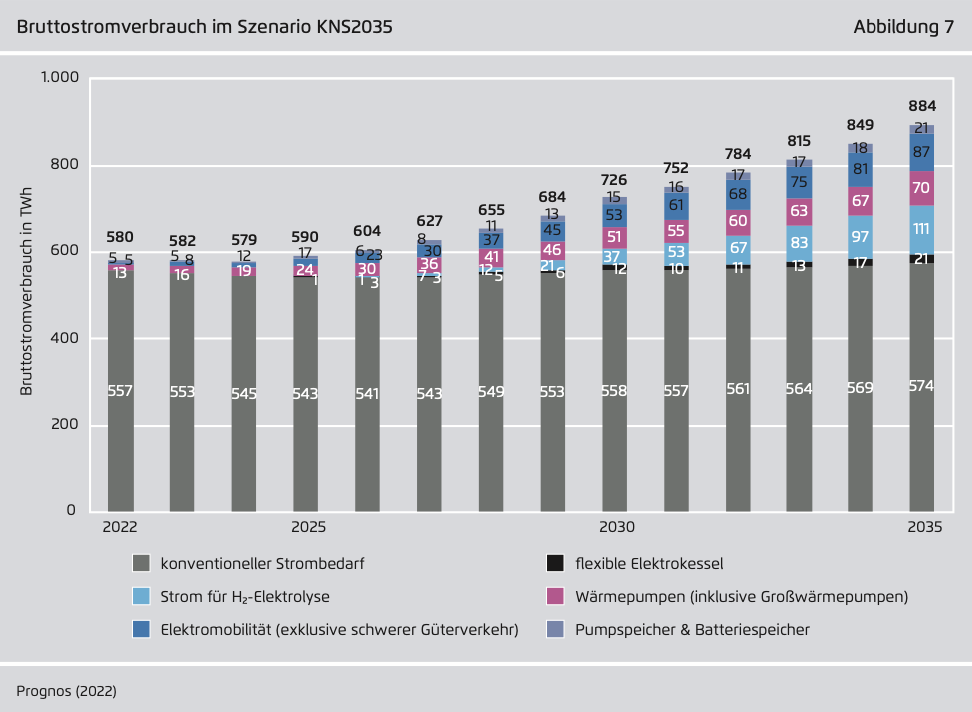
\includegraphics[page=1, clip, width=0.6\textwidth]{./anhang/Zunahme Stromverbrauch Agora2035.png}
				\caption{Zunahme des Stromverbrauchs bietet gleichzeitig Flexibilität}
				\label{Abb. Zunahme Flexibilität} \cite[S.33]{Agora_KlimaneutralesStromsystem}
			\end{figure}
		
		Insgesamt ist in Abbildung \ref{Abb. Zunahme Flexibilität} erkennbar, dass der steigende Stromverbrauch gleichzeitig der Flexibilität des Stromnetzes dient und so die Nutzung erneuerbarer und dargebotsabhäniger Energien maximiert.\\
		
		\subsubsection{Entwicklung der Reserve bis 2045}
		In diesem Absatz soll es um die Weiterentwicklung des Stromsektors bis 2045 gehen. Die Bundesregierung hat das Ziel geäußert bis zu diesem Jahr die Klimaneutralität zu erlangen.\\
		Folgend wird, Bezugnehmend auf das Kapitel 2 der Studie "`Energiewende im Sozialen Raum"', ein Pfad beschrieben mit dem Deutschland die Klimaneutralität 2045 erreichen kann. Wie auch im vorangegangenen Kapitel müssen dafür Annahmen getroffen werden. Diese wurden dem "`Ariadne-Report"' des Potsdam-Insitut für Klimafolgenforschung (PIK) entnommen.\cite[S.150]{AriadneReport} Die Ausarbeitung betrachtet das "`Fokus PV Szenario"', da davon ausgegangen wird, dass die Akzeptanz für Windkraft und Trassenausbau in der Bevölkerung konservativ bleibt.\\
		Die Studie bezieht die aktuellen Ereignisse des Ukraine-Krieges nicht mit ein und muss daher im Hinblick auf Laufzeitverlängerungen für Atom- und Kohlekraftwerke differenziert betrachtet werden.\\
		
		Basierend auf dem Modell SCOPE-Path, das die Entwicklung des künftigen europäischen Strommarktes zeigt, wird ein Szenario entwickelt, in dem das Ziel der Klimaneutralität möglichst kostenoptimiert erreicht wird.\\
		Grundlage für Stromerzeugung und -verbrauch bot das Wetterjahr 2012. Dieses zeichnet sich speziell durch eine lange Kälteperiode und niedrige Erträge aus Windkraft aus. Damit soll indirekt auch die Versorgungssicherheit betrachtet werden.\cite[S.2]{ESRa_Fraunhofer}\\
		
		Die Studie bezieht sich auf ein PV-Fokussiertes Szenario. Hierbei wird auf Grund von Genehmigungen, Naturschutz, fehlender Flächenausweisung und fehlender Akzeptanz davon ausgegangen, das weniger Windkraft, dafür aber mehr Photovoltaik ausgebaut wird.\cite[S.4]{ESRa_Fraunhofer}\\
		Desweiteren soll angenommen werden, dass die Kapazitäten der Wasserkraft erschöpft sind und eine Nutzung von Geothermie für Stromerzeugung nicht wirtschaftlich ist. Der Ausbau von Biomasse ist auf Grund von Anbauflächenkonflikten und Biodiversität beschränkt, sodass sich Photovoltaik und Windenergie zu den zentralen Technologien zur Stromerzeugung durchsetzen.\cite[S.6]{ESRa_Fraunhofer}\\
		
		Der Bruttostromverbrauch steigt bis zum Jahr 2045 auf \SI{1015}{\tera \watt \hour} an.\cite[S.10]{ESRa_Fraunhofer} Zur Sicherung der Versorgung ist eine Verfünffachung der installierten PV- und Winkraftkapazitäten bis 2045 notwendig. Diese betrugen 2021 noch \SI{116}{\giga \watt} und steigen in diesem Szenario auf \SI{550}{\giga \watt} an.\cite[S.7]{ESRa_Fraunhofer}\\
		Die zur Deckung der Nachfrage benötigte Leistung von PV beläuft sich in diesem Szenario auf \SI{400}{\giga \watt} 2045, während Onshore-Windkraft 2045 \SI{130}{\giga \watt} ausmachen. Dennoch ist die Nettostromerzeugung der Winkraftanlagen auf Grund von höheren Volllaststunden etwas größer.\cite[S.7]{ESRa_Fraunhofer} Offshore-Windkraft machen in diesem Szenario \SI{40}{\giga \watt} aus, wobei jedoch nur \SI{50}{\percent} davon zur Einspeisung in das Netz genutzt werden. Die übrigen \SI{50}{\percent} werden durch Elektrolyseure für die Wasserstoffsynthese verwendet. Grund hierfür ist die angenommene geringere Akzeptanz der Bevölkerung für Stromtrassen.\cite[S.7]{ESRa_Fraunhofer}\\
		Das Szenario zeigt, dass mit nur \SI{38}{\tera \watt \hour} Stromimporten die Nachfrage fast vollständig inländisch gedeckt werden kann.\cite[S.16]{ESRa_Fraunhofer}\\
		
		Zur Deckung der Redisuallasten werden \SI{58}{\giga \watt} Gaskraftwerksleistungen vorgehalten. Diese müssen allerdings, wie in \ref{sect: 2030} schon ausgeführt, bereits 2030 installiert sein. Der Anteil von Erdgas sinkt im Laufe der Jahre weiter. 2045 werden alle Gas-KWK-Anlagen rein mit erneuerbarem Wasserstoff betrieben.\cite[S.8]{ESRa_Fraunhofer}\\
		
		Auch in diesem Szenario überwiegen flexible Lasten im Energiesystem. Power-to-heat und Power-to-hydrogen, sowie die flächendeckende Verbreitung von Elektrofahrzeugen prägen die energetische Landschaft in 2045. Der Anteil von Wärmepumpen zur Bereitung von Raumwärme steigt auf \SI{54}{\percent}, die verbliebenen Wasserstoff-Gaskessel machen noch \SI{9}{\percent} aus. Mit Power-to-heat Anlagen, wie beispielsweise Elektrodenkesseln, werden Fernwärmenetze aufgebaut um die industriellen Anforderungen nach Hochtemperaturwärme zu decken. Großwärmepumpen werden zur Niedertemperaturwärmeversorgung (unter \SI{100}{\degreeCelsius}) eingesetzt.\cite[S.10ff]{ESRa_Fraunhofer}\\ Diese Technologien dienen auch hier unter zu Hilfe nahme der Gas- und Wasserkraft als Regelreserven zur Frequenz- und Spannungshaltung.
		
				\begin{figure}[H]
				\centering
				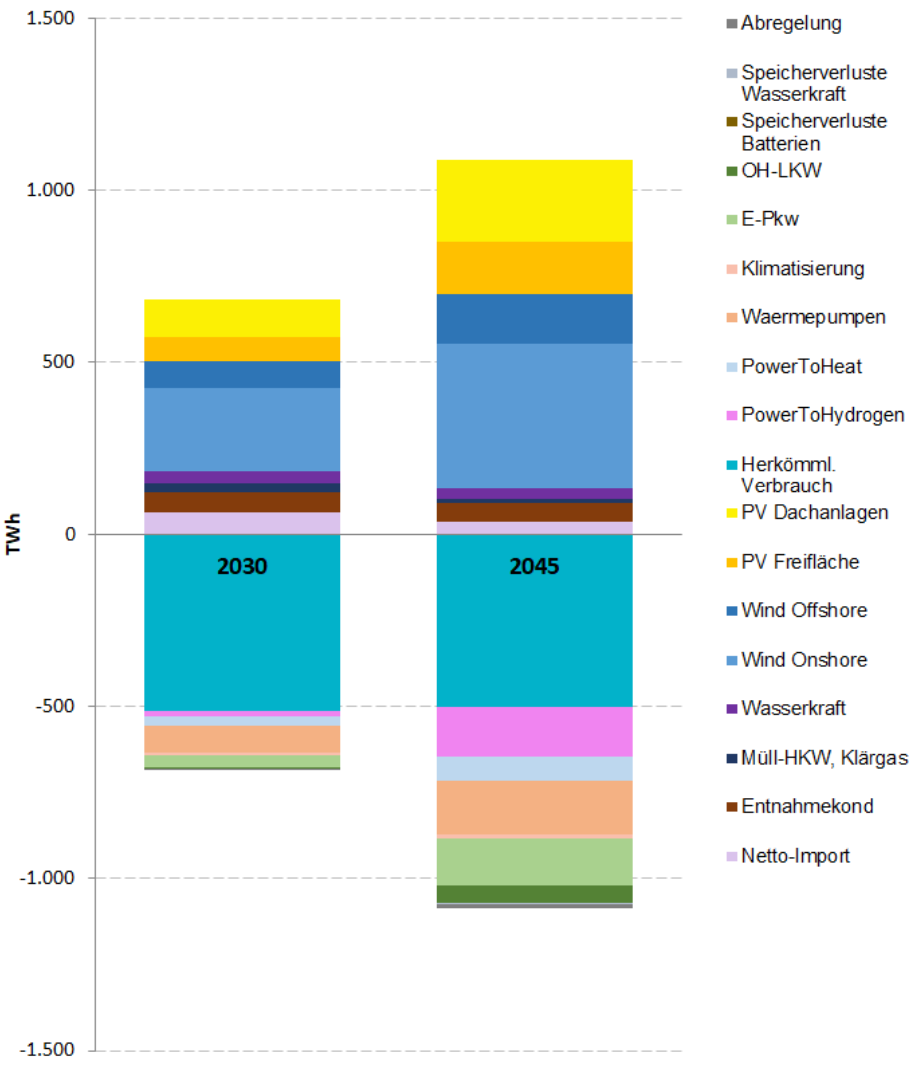
\includegraphics[page=1, clip, width=0.6\textwidth]{./anhang/Strombilanz Frauenhofer.png}
				\caption{Energieerzeugung und -verbrauch 2030 und 2045 im Vergleich}
				\label{Abb. Energiesystem 2045} \cite[S.9]{ESRa_Fraunhofer}
			\end{figure}
		
		\subsubsection{Vergleich beider Szenarien}
		Vergleicht man beide Szenarien, so stellt man fest, dass die Unterschiede, auf Grund des  PV-Fokussierten Szenarios in der Studie Energiewende im Sozialen Raum, groß sind. Während in der Ausarbeitung der Agora-Energiewende 2030 \SI{115}{\giga \watt} Onshore-Windkraft und \SI{215}{\giga \watt} PV installiert werden, sind es im Bericht "`Energiewende im Sozialen Raum"' \SI{83}{\giga \watt} Wind Onshore und \SI{185}{\giga \watt} PV. Offshore-Wind unterscheidet sich hier um \SI{18}{\giga \watt} (\SI{40}{\giga \watt} ESRa und \SI{58}{\giga \watt} Agora). Die Unterschiede in der Dimensionen des Ausbaus erneuerbarer Energien liegen in den Zielen der Studien begründet. Während die Studie von Agora-Energiewende an den momentanen Zielen der Ampel-Koalition orientiert ist, führt die Studie "`Energiewende im Sozialen Raum"' die EU-Ziele als Ausgangspunkt auf. Diese sind konservativer als es die nationalen Ziele sind.\cite{EU_Klimaziele}
		\clearpage
		
		
		